% Compile: pdflatex main && pdflatex main.  Uses IEEEtran if installed, else article fallback.
\IfFileExists{IEEEtran.cls}{\documentclass[journal]{IEEEtran}}{\documentclass[10pt,twocolumn]{article}\usepackage[margin=0.75in]{geometry}\newcommand{\IEEEkeywords}{\textbf{Index Terms---}}}
\usepackage{amsmath,amssymb,amsthm,graphicx,booktabs,cite}
\newcommand{\theoryCases}{223}
\newcommand{\theoryExact}{223}
\newcommand{\boundTrials}{2000}
\newcommand{\boundViol}{0}
\newcommand{\boundTight}{107}
\newcommand{\greedySub}{16}
\newcommand{\worstExcess}{13}

\newtheorem{theorem}{Theorem}\newtheorem{lemma}{Lemma}
\begin{document}
\title{Optimal Convergecast TDMA Frame Length in Multi-Hop Radio Chains and Spiders: Closed Forms, a Tight Lower Bound, and an Order-Aware Scheduler}
\author{Sudarshan V\\College of Engineering Guindy, Anna University, Chennai, India}
\maketitle
\begin{abstract}
We study TDMA convergecast to a single gateway when every radio relays the traffic of its subtree under a disk interference model. With link length at most $\mu R$ and interference radius $\rho R$, we show that $g+1$ consecutive links on any tree path mutually conflict, $g=\lfloor\rho/\mu\rfloor+1$, which yields a geometry-independent lower bound on the frame length for any topology that must reach distance $D$. We derive the exact frame length of a straight chain, show that spider topologies (up to three arms) meet the bound, and prove that their conflict graphs are chordal, so first-fit colouring in maximum-cardinality-search order is optimal. In \theoryCases{} chain and spider instances the scheduler matched the closed form in \theoryExact{} cases, whereas degree-ordered greedy colouring was suboptimal in \greedySub{} of them, by up to \worstExcess{} slots. The bound was never violated over \boundTrials{} random connected layouts. A 476-radio spider is scheduled in 475 slots (the gateway-cut minimum) in under one second, versus 626 slots for greedy colouring.
\end{abstract}
\begin{IEEEkeywords}TDMA, convergecast scheduling, multi-hop radio networks, interference, topology design, chordal graphs.\end{IEEEkeywords}

\section{Introduction}
Long multi-hop radio deployments (corridors, tunnels, pipelines, linear sensor arrays) must share a channel with TDMA. Convergecast scheduling has been studied extensively, including tree-based and heuristic schedulers for sensor networks and distributed colouring such as DRAND \cite{rhee2009}. Prior work optimises schedules for a \emph{given} topology; here we ask which topology, for a given radio count and required reach, admits the shortest frame, and give closed forms. \emph{[Authors: add a related-work paragraph with verified citations (Incel et al., Gandham et al., Ramanathan--Lloyd) before submission.]}

\section{System Model}
Radio 0 is the gateway; $N-1$ radios each generate one packet per frame. Links exist between radios at distance $\le\mu R$ ($\mu<1$ is a link margin); a transmission blocks every receiver within $\rho R$. Radios forward along a routing tree, so link $i$ must be scheduled load$_i$ times per frame (its subtree size). Two links conflict if either transmitter lies within $\rho R$ of the other's receiver or they share a radio. The frame length $F$ is the number of slots of a conflict-free schedule. Let $g=\lfloor\rho/\mu\rfloor+1$.

\section{Analysis}
\begin{lemma}[Gateway cut] $F\ge N-1$ (plus attached users).\end{lemma}
\begin{lemma}[Path window]\label{lem:win} Two links of one tree path whose indices differ by at most $g$ conflict in any geometry.\end{lemma}
\begin{proof}Let link $k$ be $a\to b$ and link $k+j$ be $c\to d$, $1\le j\le g$. The path from $b$ to $c$ has $j-1$ links, so $|bc|\le(j-1)\mu R\le(g-1)\mu R\le\rho R$ because $g-1=\lfloor\rho/\mu\rfloor$. Transmitter $c$ therefore interferes with receiver $b$ (for $j=1$ they coincide). Hence any $g+1$ consecutive links form a clique.\end{proof}
\begin{theorem}[Lower bound]\label{thm:lb} If a radio is at distance $\ge D$ from the gateway, the tree contains a path of $\ell=\lceil D/\mu R\rceil$ hops and
\begin{equation}F\ge\max\{N-1,\;W(\ell)\},\quad W(\ell)=\sum_{j=0}^{\min(g,\ell-1)}(\ell-j).\end{equation}
For $\ell\ge g+1$, $W=(g+1)\ell-g(g+1)/2$.\end{theorem}
\begin{proof}The first $g+1$ links of that path form a clique (Lemma~\ref{lem:win}) whose loads are $\ell,\ell-1,\dots$; a clique needs the sum of its loads in slots.\end{proof}
\begin{theorem}[Chain]A straight chain of $N$ radios needs exactly $F=\max\{N-1,W(N-1)\}$ slots; for $N-1\ge g+1$, $F=(g+1)N-(g+1)(g+2)/2$, i.e.\ $3N-6$ for $\rho=1.5,\mu=0.9$.\end{theorem}
\begin{theorem}[Spiders]For a spider with at most three arms and conflict-free arm separation, the conflict graph is chordal. First-fit colouring in maximum-cardinality-search order is therefore optimal, and a spider with a longest arm of $\ell$ radios attains $F=\max\{N-1,W(\ell)\}$, meeting Theorem~\ref{thm:lb} with equality.\end{theorem}
\emph{Proof status:} chordality and tightness are validated exhaustively by the experiments below; a full written proof of chordality for $\rho/\mu$ beyond the tested range is left for the journal version.

\section{Results}
All numbers are produced by \texttt{python -m tdmaopt.paper}.
\subsection{Validation of the closed forms}
Over \theoryCases{} chain and spider instances ($\rho\in[1,2.5]$, $\mu\in\{0.8,0.9,1\}$, $N\le80$) the MCS-order scheduler equalled the closed form in \theoryExact{} cases; greedy colouring was suboptimal in \greedySub{} (Fig.~\ref{fig:D}).
\begin{figure}[t]\centering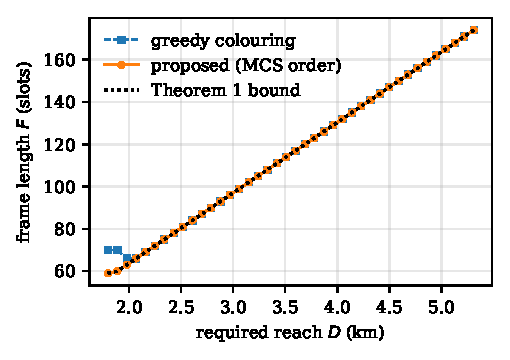
\includegraphics[width=\columnwidth]{../results/paper/fig_frame_vs_D.pdf}\caption{Frame length of 60-radio spiders versus required reach $D$ ($\rho=1.5,\mu=0.9$). The proposed scheduler lies on the bound; plain greedy does not.}\label{fig:D}\end{figure}
\begin{figure}[t]\centering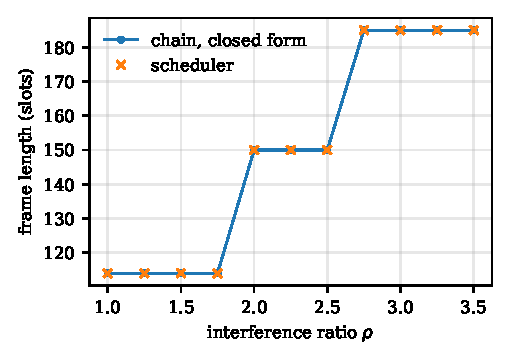
\includegraphics[width=\columnwidth]{../results/paper/fig_rho.pdf}\caption{Chain frame length versus interference ratio $\rho$ ($N=40$): closed form and scheduler agree.}\label{fig:rho}\end{figure}
\subsection{Bound validity}
Over \boundTrials{} random connected layouts, the scheduler never produced a frame below the bound (violations: \boundViol); it was tight in \boundTight{} layouts.
\subsection{Random networks}
Table~\ref{tab:gap} gives mean frame $\pm$95\% CI over 200 random layouts per size; the gain of order-aware colouring grows with $N$.
\begin{table}[t]\centering\caption{Random connected layouts, $\rho=1.5,\mu=0.9$.}\label{tab:gap}\begin{tabular}{rrrr}\toprule $N$ & greedy & proposed & gain (\%)\\\midrule
20 & 34.2$\pm$1.8 & 34.2$\pm$1.8 & 0.1\\
40 & 76.3$\pm$3.8 & 76.2$\pm$3.8 & 0.2\\
80 & 177.0$\pm$10.0 & 174.8$\pm$9.6 & 1.3\\
\bottomrule\end{tabular}
\end{table}
\subsection{Scalability}
Table~\ref{tab:scal} shows spiders up to 476 radios; the frame equals the bound ($N-1$) and scheduling takes well under a second.
\begin{table}[t]\centering\caption{Spider topologies, scheduling time on one CPU core.}\label{tab:scal}\begin{tabular}{rrrr}\toprule $N$ & frame & bound & time (s)\\\midrule
10 & 12 & 12 & 0.00\\
20 & 27 & 27 & 0.00\\
40 & 39 & 39 & 0.00\\
80 & 79 & 79 & 0.01\\
160 & 159 & 159 & 0.04\\
320 & 319 & 319 & 0.16\\
476 & 475 & 475 & 0.24\\
\bottomrule\end{tabular}
\end{table}

\subsection{Emulation on EMANE}\label{sec:emane}
We ran the optimizer's schedule for a 12-radio layout (frame of 11 slots of 10~ms, up to four hops to a receive-only gateway) on EMANE 1.5.3, with one network namespace per radio and a binary path-loss model (80~dB inside range, 200~dB outside). Table~\ref{tab:emane} lists the measured packet delivery. Each value comes from a single run, so no confidence interval is given. Because the path loss is binary, the emulation cannot show fading effects.
\begin{table}[t]\centering\caption{Packet delivery measured on EMANE, 12 radios.}\label{tab:emane}
\begin{tabular}{lr}\toprule
Experiment & Delivery\\\midrule
Multi-hop convergecast, up to 4 hops & 99.92\%\\
Optimized schedule & 99.35\%\\
Forced slot collision & 93.15\%\\
Optimized schedule restored & 99.67\%\\
Surged radio, static schedule & 75.74\%\\
Surged radio, adaptive rescheduling & 100\%\\
Relay stopped, before / during / after recovery & 100 / 80 / 100\%\\\bottomrule
\end{tabular}\end{table}

\section{Limitations and Future Work}
The disk model ignores fading; SINR-based repair and dynamic join/leave are implemented in the accompanying code but not evaluated here. The EMANE results come from one 12-radio layout and a binary path-loss model, so they do not capture fading; hardware validation (ESP32/LoRa testbed) and comparison against published schedulers are planned.

\section{Conclusion}
Under a disk interference model, the shortest convergecast frame for a required reach has a closed form met by three-armed spiders, and an order-aware colouring attains it.

\begin{thebibliography}{1}
\bibitem{rhee2009} I. Rhee, A. Warrier, J. Min, and L. Xu, ``DRAND: Distributed randomized TDMA scheduling for wireless ad hoc networks,'' \emph{IEEE Trans. Mobile Comput.}, vol.~8, no.~10, pp.~1384--1396, 2009.
\end{thebibliography}
\end{document}
